\documentclass[11pt,letterpaper]{article}
\usepackage{anysize}
\usepackage{indentfirst}
\usepackage{sectsty}
\usepackage{amsmath}
\usepackage{hyperref}
\usepackage{graphicx}
\usepackage{chngpage}
\usepackage{enumerate}
\hypersetup{
	colorlinks=true, 
	linkcolor=blue, 
	urlcolor=blue, 
	pdfnewwindow=true, 
	citecolor=black
}
\urlstyle{same}
\linespread{1.2}

\begin{document}

\begin{titlepage}
    \vspace*{4cm}
    \begin{flushright}
    {\huge
        Project 2\\[5mm]
    }
    {\large
        CS325 | Spring 2015
     }
    \end{flushright}
\hrule
    \begin{flushright}
	by Group 2\\
	Vedanth Narayanan\\
	Jonathan Merrill\\
	Tracie Lee\\
    \vfill
	\today\\
    \end{flushright}
\end{titlepage}

\raggedright

\section{Dynamic Programming Table}
Starting with i = 0 and incrementing to the amount of change passed in, we fill in the table with the minimum number of coins needed to make i cents. As i increases, we use previous smaller values that are stored in the table to compute the minimum number of coin for i cents. By building the table from the smallest values to the largest, we can reuse the work to find optimal numbers of coins for each iteration until we eventually get to the value passed in. 
\section{Algorithm Pseudocode}
\begin{verbatim}
-- Divide and Conquer --

Define changeslowhelper(currency[], amount)
    // currency = array of coin denominations
    // amount = int, total amount we're making change for
    
    if amount == 0
        return 0
    for each coin in currency
        if coin == amount
            return [coin]
			
    for i to amount/2
        temp.extend(changeslowhelper(currency, i))
        temp.extend(changeslowhelper(currency, amount - 1))
        numCoins = length of temp
		
        if numCoins < minCoins
            coins = temp
	
    return coins
	
Define changeslow(currency[], amount)
    coins = changeslowhelper(currency[], amount)
	
    for each coin in currency
        result.append(coins.count(coin))
	
    return result
	
===================================================================================
===================================================================================
-- Greedy --

Define changegreedy (currency[], amount)
    int num
	
    for i to currency.length
		
        if currency[i] <= amount
            num = amount / currency[i]
            numArray[i] = numArray[i] + num
            total = total + num
            amount -= num * currency[i]
	
    numArray.append(total)  // sending the total through on the end of the array
                            // then we'll strip it off in the print function
    return numArray
    
===================================================================================
===================================================================================
-- Dynamic Programming --

Define changedp (currency[], amount)
    table[0] = 0
    table2[0] = 0
    for j from 1 to amount 
        for i from 0 to len(currency)
            if currency[i] <= j
                min = 1 + table[j - currency[i]]
                coin = i
        append min to table
        append coin to table2

    coins = []
    while amount > 0
        append table2[amount] to result
        decrement amount by table2[amount]
	
    result = []
    for each coin in currency
	    append the number of each coin in coins to result
		
    return result

\end{verbatim}

\section{Dynamic Programming Induction Proof}
	Proof by Induction:
\begin{itemize}
	\item \textbf{Base Case}\\
	T[0] = 0. This is true because for 0 cents, the optimal number of coins used is 0.
	\item \textbf{Inductive Hypothesis}\\
	We assume that for some arbitrary value 'k', T[k] is the minimum number of coins used to make change for k cents. This also assumes that T[p] is correct, where p is any value less than or equal to k, due to the nature of the problem.
	\item \textbf{Inductive Step}\\
	We must now prove that T[k+1] is also correct:\\
	\hspace{15pt}Since:\\ 
	\hspace{30pt}T[k+1] = T[(k+1) - i] + 1; where i is some value less than or equal to k\\
	\hspace{15pt}Then:\\
	\hspace{30pt}T[k+1] = T[p] + 1; where p is some value less than or equal to k\\
	Since we know T[p] is the correct number of coins used for p cents, T[k+1] must also be the correct number of coins used for k+1 cents.
\end{itemize}	 
\section{Greedy and DP Algorithms for V = [1, 5, 10, 25, 50]}
	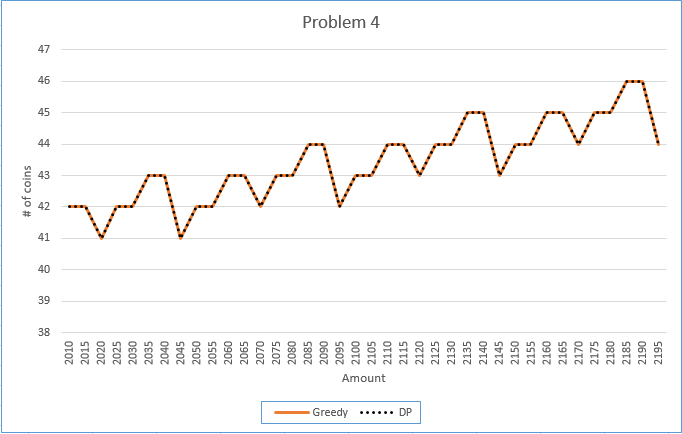
\includegraphics[width=6in]{p4.png}\\
	As you can see, both algorithms are identical in the results produced for V = [1,5,10,25,50].\\
\section{Greedy and DP Algorithms for V = [1, 2, 6, 12, 24, 48, 60] and V = [1, 6, 13, 37, 150]}
	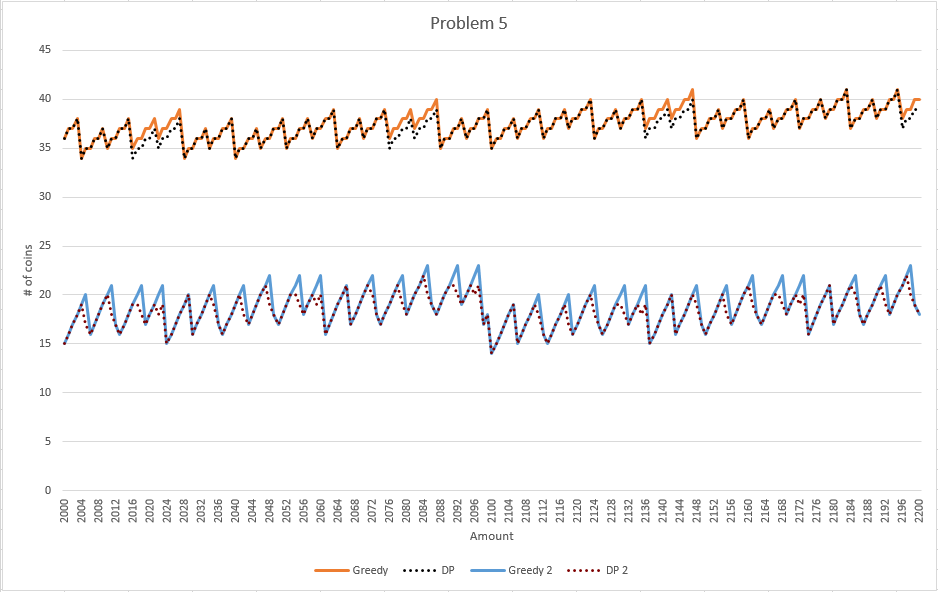
\includegraphics[width=6in]{p5.png}\\
	For some values in the Dynamic Programming algorithm, more minimized results are returned in comparison to the greedy algorithm. This is true for both V = [1, 2, 6, 12, 24, 48, 60] and V = [1, 6, 13, 37, 150].\\
\section{Greedy and DP Algorithms for V = [1, 2, 4, 6, 8, 10, 12, ..., 30]}
	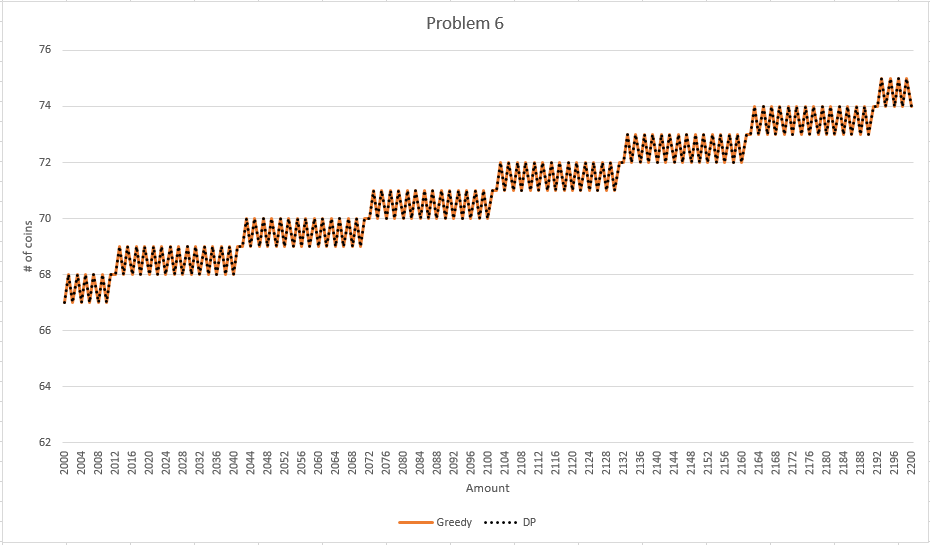
\includegraphics[width=5.5in]{p6.png}\\
	As you can see, both algorithms are identical in the results produced for V = [1, 2, 4, 6, 8, 10, 12, ..., 30].\\
\section{Running Times for Greedy and DP Algorithms}
	\textbf{Problem 4}\\
	\hskip-1.0cm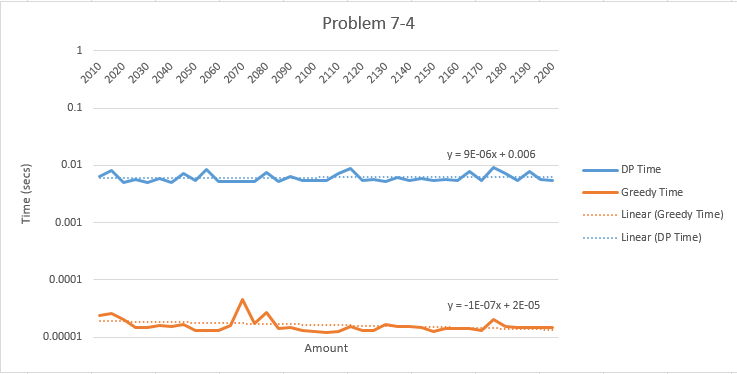
\includegraphics[width=6.5in]{p7-4.png}\\
	\textbf{Problem 5}\\
	\hskip-1.0cm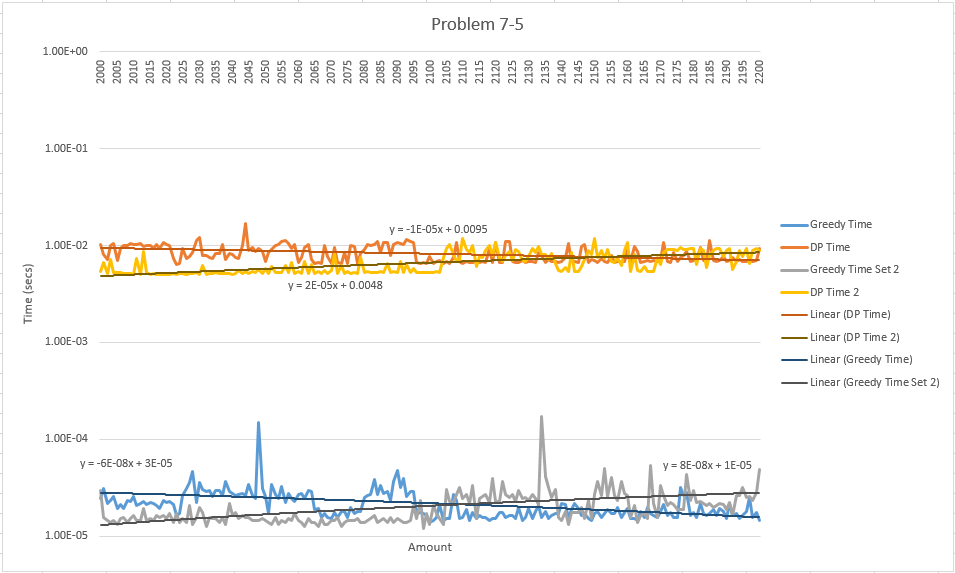
\includegraphics[width=6.5in]{p7-5.png}\\
	\textbf{Problem 6}\\
	\hskip-1.0cm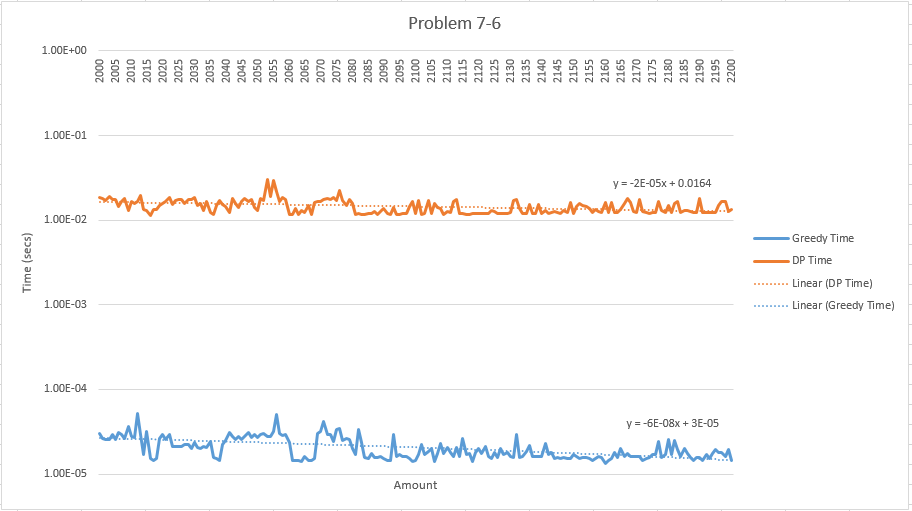
\includegraphics[width=6.5in]{p7-6.png}\\
	
\section{Running Times vs Number of Denominations for Greedy and DP Algorithms}
	\hskip-1.0cm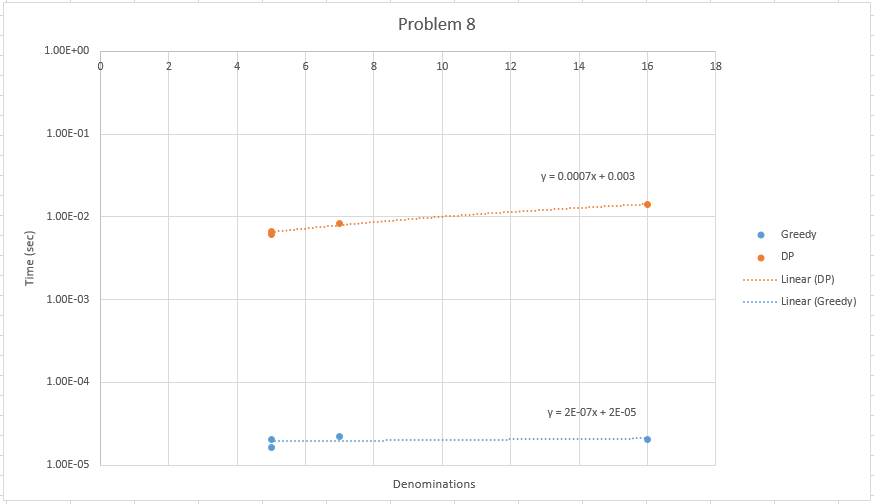
\includegraphics[width=6.5in]{p8.png}\\
	The number of denominations (n) influences the running times of the two algorithms. The difference would be more prevalent with larger values for n.

\section{Greedy vs DP for  V = [$p^0$, $p^1$, $p^2$, ... , $p^n$]}
	The greedy algorithm will definitely operate faster because it looks for the largest element in V that it can subtract from A, where DP will check for all elements in V.

\end{document}
